\documentclass[a4paper]{report}
\input{header}
\begin{document}
\pagestyle{noweb}

\title{\ty{gemi}: Genomik zum Mitmachen\\\small Tag der Offenen Tür am
  Max-Planck-Institut für Evolutionsbiologie\\\scriptsize \ty{github.com/eovlbioinf/gemi}}
\author{Beatriz Vieira Mourato \& Bernhard Haubold}
\date{\input{date.txt}\hspace{-3pt}, \input{version.txt}}
\maketitle

\tableofcontents

\chapter{Einleitung}\label{ch:intro}
In der Bioinformatik geht es um die Analyse biologischer Daten mit dem
Computer. Die Daten stammen meistens aus der Genomik, zum Beispiel
Genomsequenzen. In unserem kleinen Praktikum heute untersuchen wir das
Genom des Lebewesens mit dem kleinsten Genom, das Bakterium
\emph{Mycoplasmoides genitalium}, das schmerzhafte
Harnleiterinfektionen beim Menschen verursachen kann.

Unser Handwerkszeug für diese Untersuchung ist die Unix
Befehlszeile. Sie steht sie auf allen PC-Betriebssystemen zur
Verfügung, Du solltest sie jetzt vor dir haben.

\chapter{Die Unix Befehlszeile}\label{ch:unix}
\nwfilename{}\nwbegindocs{0}\nwenddocs{}\nwbegindocs{1}\nwdocspar% ===> this file was generated automatically by noweave --- better not edit it
Zu Beginn laden wir laden wir das Repo \ty{gemi} für \emph{Genomik zum
Mitmachen} herunter.
\nwenddocs{}\nwbegincode{2}\sublabel{NW0-3RVIge-1}\nwmargintag{{\nwtagstyle{}\subpageref{NW0-3RVIge-1}}}\moddef{unix.sh~{\nwtagstyle{}\subpageref{NW0-3RVIge-1}}}\endmoddef\nwstartdeflinemarkup\nwprevnextdefs{\relax}{NW0-3RVIge-2}\nwenddeflinemarkup
git clone https://github.com/evolbioinf/gemi
\nwalsodefined{\\{NW0-3RVIge-2}\\{NW0-3RVIge-3}\\{NW0-3RVIge-4}\\{NW0-3RVIge-5}}\nwnotused{unix.sh}\nwendcode{}\nwbegindocs{3}\nwdocspar
Wir wechseln in das neue Verzeichnis, \ty{gemi}.
\nwenddocs{}\nwbegincode{4}\sublabel{NW0-3RVIge-2}\nwmargintag{{\nwtagstyle{}\subpageref{NW0-3RVIge-2}}}\moddef{unix.sh~{\nwtagstyle{}\subpageref{NW0-3RVIge-1}}}\plusendmoddef\nwstartdeflinemarkup\nwprevnextdefs{NW0-3RVIge-1}{NW0-3RVIge-3}\nwenddeflinemarkup
cd gemi
\nwendcode{}\nwbegindocs{5}\nwdocspar
Wir listen die Dateien und Verzeihnise in \ty{gemi}.
\nwenddocs{}\nwbegincode{6}\sublabel{NW0-3RVIge-3}\nwmargintag{{\nwtagstyle{}\subpageref{NW0-3RVIge-3}}}\moddef{unix.sh~{\nwtagstyle{}\subpageref{NW0-3RVIge-1}}}\plusendmoddef\nwstartdeflinemarkup\nwprevnextdefs{NW0-3RVIge-2}{NW0-3RVIge-4}\nwenddeflinemarkup
ls
\nwendcode{}\nwbegindocs{7}\nwdocspar
Wir wechseln in das Verzeichnis \ty{spielplatz}.
\nwenddocs{}\nwbegincode{8}\sublabel{NW0-3RVIge-4}\nwmargintag{{\nwtagstyle{}\subpageref{NW0-3RVIge-4}}}\moddef{unix.sh~{\nwtagstyle{}\subpageref{NW0-3RVIge-1}}}\plusendmoddef\nwstartdeflinemarkup\nwprevnextdefs{NW0-3RVIge-3}{NW0-3RVIge-5}\nwenddeflinemarkup
cd spielplatz
\nwendcode{}\nwbegindocs{9}\nwdocspar
Wir listen die Dateien in \ty{spielplatz}.
\nwenddocs{}\nwbegincode{10}\sublabel{NW0-3RVIge-5}\nwmargintag{{\nwtagstyle{}\subpageref{NW0-3RVIge-5}}}\moddef{unix.sh~{\nwtagstyle{}\subpageref{NW0-3RVIge-1}}}\plusendmoddef\nwstartdeflinemarkup\nwprevnextdefs{NW0-3RVIge-4}{\relax}\nwenddeflinemarkup
ls
\nwendcode{}

\nwixlogsorted{c}{{unix.sh}{NW0-3RVIge-1}{\nwixd{NW0-3RVIge-1}\nwixd{NW0-3RVIge-2}\nwixd{NW0-3RVIge-3}\nwixd{NW0-3RVIge-4}\nwixd{NW0-3RVIge-5}}}%


\chapter{Gene}\label{ch:latex}
\nwfilename{}\nwbegindocs{0}\nwenddocs{}\nwbegindocs{1}\nwdocspar% ===> this file was generated automatically by noweave --- better not edit it
Wir möchten das Genom von \emph{Mycoplasmoides genitalium}
untersuchen. Genauer gesagt, das Genom des \emph{Typstamms} von
\emph{M. genitalium}, G37. Dazu benötigen wir die Taxon-ID von
\emph{M. genitalium} G37. Die schauen wir mit dem Programm \ty{taxi}
in einer \emph{remoten} Datenbank nach, \ty{-r}. Wir finden heraus,
die Taxon-ID von \emph{M. genitalium} ist 243273.
\nwenddocs{}\nwbegincode{2}\sublabel{NW0-2qU5iO-1}\nwmargintag{{\nwtagstyle{}\subpageref{NW0-2qU5iO-1}}}\moddef{gene.sh~{\nwtagstyle{}\subpageref{NW0-2qU5iO-1}}}\endmoddef\nwstartdeflinemarkup\nwprevnextdefs{\relax}{NW0-2qU5iO-2}\nwenddeflinemarkup
taxi -r "genitalium G37"
\nwalsodefined{\\{NW0-2qU5iO-2}\\{NW0-2qU5iO-3}\\{NW0-2qU5iO-4}\\{NW0-2qU5iO-5}\\{NW0-2qU5iO-6}\\{NW0-2qU5iO-7}\\{NW0-2qU5iO-8}\\{NW0-2qU5iO-9}\\{NW0-2qU5iO-A}\\{NW0-2qU5iO-B}\\{NW0-2qU5iO-C}\\{NW0-2qU5iO-D}\\{NW0-2qU5iO-E}\\{NW0-2qU5iO-F}\\{NW0-2qU5iO-G}\\{NW0-2qU5iO-H}\\{NW0-2qU5iO-I}\\{NW0-2qU5iO-J}\\{NW0-2qU5iO-K}\\{NW0-2qU5iO-L}\\{NW0-2qU5iO-M}\\{NW0-2qU5iO-N}\\{NW0-2qU5iO-O}\\{NW0-2qU5iO-P}\\{NW0-2qU5iO-Q}\\{NW0-2qU5iO-R}\\{NW0-2qU5iO-S}\\{NW0-2qU5iO-T}\\{NW0-2qU5iO-U}\\{NW0-2qU5iO-V}\\{NW0-2qU5iO-W}\\{NW0-2qU5iO-X}\\{NW0-2qU5iO-Y}\\{NW0-2qU5iO-Z}\\{NW0-2qU5iO-a}\\{NW0-2qU5iO-b}\\{NW0-2qU5iO-c}\\{NW0-2qU5iO-d}\\{NW0-2qU5iO-e}\\{NW0-2qU5iO-f}}\nwnotused{gene.sh}\nwendcode{}\nwbegindocs{3}\nwdocspar
\begin{verbatim}
# ID      Parent  Name
243273  2097    Mycoplasmoides genitalium G37
\end{verbatim}
\nwenddocs{}\nwbegindocs{4}\nwdocspar
Genome werden durch \emph{Accessions} identifiziert. Mit Hilfe der
Taxon-ID können wir die Accessions der Genome von \emph{M. genitalium}
G37 nachsehen. Dazu verwenden wir das Programm \ty{neighbors}, dem wir
wieder \emph{remote} (\ty{-r}) als \emph{target} die Taxon-ID geben
(\ty{-t}) und nur die Genome dieser Targets anfordern (\emph{only},
\ty{-o}). Die Genome sollen Qualitäts-\emph{Level} (\ty{-L})
\emph{complete} sein. Wir bekommen ein Genome angeboten,
GCF\_000027325.1.
\nwenddocs{}\nwbegincode{5}\sublabel{NW0-2qU5iO-2}\nwmargintag{{\nwtagstyle{}\subpageref{NW0-2qU5iO-2}}}\moddef{gene.sh~{\nwtagstyle{}\subpageref{NW0-2qU5iO-1}}}\plusendmoddef\nwstartdeflinemarkup\nwprevnextdefs{NW0-2qU5iO-1}{NW0-2qU5iO-3}\nwenddeflinemarkup
neighbors -r -t 243273 -o -L complete
\nwendcode{}\nwbegindocs{6}\nwdocspar
\small
\begin{verbatim}
# MRCA(targets): 243273, Mycoplasmoides genitalium G37
# MRCA(targets+neighbors): 243273, Mycoplasmoides genitalium G37
# Type  Taxon-ID  Name                           Genomes
t       243273    Mycoplasmoides genitalium G37  GCF_000027325.1
\end{verbatim}
\normalsize

Wir laden das eben gefundene Genom vom Netz mit dem Programm
\ty{datasets}, zusammen mit den Gen-Annotationen im sogenannten
GFF3-Format.
\nwenddocs{}\nwbegincode{7}\sublabel{NW0-2qU5iO-3}\nwmargintag{{\nwtagstyle{}\subpageref{NW0-2qU5iO-3}}}\moddef{gene.sh~{\nwtagstyle{}\subpageref{NW0-2qU5iO-1}}}\plusendmoddef\nwstartdeflinemarkup\nwprevnextdefs{NW0-2qU5iO-2}{NW0-2qU5iO-4}\nwenddeflinemarkup
datasets download genome accession GCF_000027325.1 \\
         --include genome,gff3
\nwendcode{}\nwbegindocs{8}\nwdocspar
Wir haben jetzt die gezippte, also komprimierte Datei
\ty{ncbi\_dataset.zip} heruntergeladen.
\nwenddocs{}\nwbegincode{9}\sublabel{NW0-2qU5iO-4}\nwmargintag{{\nwtagstyle{}\subpageref{NW0-2qU5iO-4}}}\moddef{gene.sh~{\nwtagstyle{}\subpageref{NW0-2qU5iO-1}}}\plusendmoddef\nwstartdeflinemarkup\nwprevnextdefs{NW0-2qU5iO-3}{NW0-2qU5iO-5}\nwenddeflinemarkup
ls
\nwendcode{}\nwbegindocs{10}\nwdocspar
Wir entzippen die Datei.
\nwenddocs{}\nwbegincode{11}\sublabel{NW0-2qU5iO-5}\nwmargintag{{\nwtagstyle{}\subpageref{NW0-2qU5iO-5}}}\moddef{gene.sh~{\nwtagstyle{}\subpageref{NW0-2qU5iO-1}}}\plusendmoddef\nwstartdeflinemarkup\nwprevnextdefs{NW0-2qU5iO-4}{NW0-2qU5iO-6}\nwenddeflinemarkup
unzip ncbi_dataset.zip
\nwendcode{}\nwbegindocs{12}\nwdocspar
Die neuen Daten liegen jetzt in einem Unter-Unterverzeichnis von
\ty{ncbi\_dataset}. Um die Eingabe langer Verzeichnisnamen zu
vereinfachen, kann man die Selbst-Vervollständigung verwenden: Man
tippt die ersten paar Buchstaben eines Namens, gefolgt von
\ty{Tab}. Wenn der Rest des Namens eindeutig ist, wird er
hingeschrieben. Wenn nicht, bekommt man beim zweiten \ty{Tab} die
Möglichkeiten angezeigt.
\nwenddocs{}\nwbegincode{13}\sublabel{NW0-2qU5iO-6}\nwmargintag{{\nwtagstyle{}\subpageref{NW0-2qU5iO-6}}}\moddef{gene.sh~{\nwtagstyle{}\subpageref{NW0-2qU5iO-1}}}\plusendmoddef\nwstartdeflinemarkup\nwprevnextdefs{NW0-2qU5iO-5}{NW0-2qU5iO-7}\nwenddeflinemarkup
ls ncbi_dataset/data/GCF_000027325.1/
\nwendcode{}\nwbegindocs{14}\nwdocspar
Um uns die Arbeit zu erleichtern, kopieren wir die beiden Dateien zu
enfacheren Namen mit dem Befehl \ty{cp} für \emph{copy}. Zuerst das
Genom zu \ty{genom.fna}. Das Anhängsel \ty{fna} bedeutet Nukleotide im
FASTA Format. Das FASTA Format ist ein weitverbreitetes Format für
Sequenzen. Wir werden es gleich noch sehen.  \tiny
\nwenddocs{}\nwbegincode{15}\sublabel{NW0-2qU5iO-7}\nwmargintag{{\nwtagstyle{}\subpageref{NW0-2qU5iO-7}}}\moddef{gene.sh~{\nwtagstyle{}\subpageref{NW0-2qU5iO-1}}}\plusendmoddef\nwstartdeflinemarkup\nwprevnextdefs{NW0-2qU5iO-6}{NW0-2qU5iO-8}\nwenddeflinemarkup
cp ncbi_dataset/data/GCF_000027325.1/GCF_000027325.1_ASM2732v1_genomic.fna genom.fna
\nwendcode{}\nwbegindocs{16}\nwdocspar
\normalsize
Dann die Annotationen zu \ty{annotation.gff}.
\tiny
\nwenddocs{}\nwbegincode{17}\sublabel{NW0-2qU5iO-8}\nwmargintag{{\nwtagstyle{}\subpageref{NW0-2qU5iO-8}}}\moddef{gene.sh~{\nwtagstyle{}\subpageref{NW0-2qU5iO-1}}}\plusendmoddef\nwstartdeflinemarkup\nwprevnextdefs{NW0-2qU5iO-7}{NW0-2qU5iO-9}\nwenddeflinemarkup
cp ncbi_dataset/data/GCF_000027325.1/genomic.gff annotation.gff
\nwendcode{}\nwbegindocs{18}\nwdocspar
\normalsize
Die beiden letzten Kopier-Befehle sahen sehr ähnlich aus. Da wäre es
nützlich, wenn wir einen alten Befehl leicht wiederholen könnten. Mit
den Pfeiltasten $\uparrow$ und $\downarrow$ könnten wir in der Liste
vergangener Befehle rauf und runter laufen.

Als nächstes schauen wir uns den Kopf, \emph{head}, der Genomdatei
an. Wir sehen das FASTA Format, das besteht aus einer Kopfzeile, die
mit \verb+>+ anfängt, und einer oder mehreren Zeilen mit Sequenzdaten.
\nwenddocs{}\nwbegincode{19}\sublabel{NW0-2qU5iO-9}\nwmargintag{{\nwtagstyle{}\subpageref{NW0-2qU5iO-9}}}\moddef{gene.sh~{\nwtagstyle{}\subpageref{NW0-2qU5iO-1}}}\plusendmoddef\nwstartdeflinemarkup\nwprevnextdefs{NW0-2qU5iO-8}{NW0-2qU5iO-A}\nwenddeflinemarkup
head genom.fna
\nwendcode{}\nwbegindocs{20}\nwdocspar
\begin{verbatim}
>NC_000908.2 Mycoplasmoides genitalium G37, complete sequence
TAAGTTATTATTTAGTTAATACTTTTAACAATATTATTAAGGTATTTAAAAAATACTATTATAGTATTTAACATAGTTAA
...
\end{verbatim}
\nwenddocs{}\nwbegindocs{21}\nwdocspar
Wie den Kopf der Datei, können wir uns auch ihr anderes Ende, den
Schwanz, ansehen.
\nwenddocs{}\nwbegincode{22}\sublabel{NW0-2qU5iO-A}\nwmargintag{{\nwtagstyle{}\subpageref{NW0-2qU5iO-A}}}\moddef{gene.sh~{\nwtagstyle{}\subpageref{NW0-2qU5iO-1}}}\plusendmoddef\nwstartdeflinemarkup\nwprevnextdefs{NW0-2qU5iO-9}{NW0-2qU5iO-B}\nwenddeflinemarkup
tail genom.fna
\nwendcode{}\nwbegindocs{23}\nwdocspar
\begin{verbatim}
...
TCAAGAATGACTTTTCGCCTTTCTGGACAAAGTTTAACCAATGATCCTGCAACATTAGTTGCCATTGTAGTTTTTAATAC
GCCGCCTTTATTATTTACAAAAGAAATGATCATATATTTAAATGATTATAATATTTCTTTAATACTAAAAAAATAC
\end{verbatim}
Wir zählen die 580,076 Nukleotide im Genom von \emph{M. genitalium}.
\nwenddocs{}\nwbegincode{24}\sublabel{NW0-2qU5iO-B}\nwmargintag{{\nwtagstyle{}\subpageref{NW0-2qU5iO-B}}}\moddef{gene.sh~{\nwtagstyle{}\subpageref{NW0-2qU5iO-1}}}\plusendmoddef\nwstartdeflinemarkup\nwprevnextdefs{NW0-2qU5iO-A}{NW0-2qU5iO-C}\nwenddeflinemarkup
cres genom.fna
\nwendcode{}\nwbegindocs{25}\nwdocspar
\begin{verbatim}
Total: 580076
Residue Count  Fraction 
A       200544 0.346    
C       91515  0.158    
G       92306  0.159    
T       195711 0.337    
\end{verbatim}
\nwenddocs{}\nwbegindocs{26}\nwdocspar
Wir schauen uns den Kopf der Annotationsdatei an, aber diesmal lassen
wir uns die ersten 20 Zeilen anzeigen (\ty{-n}). Nach den
Kommentar-Zeilen mit Hash-Tag sehen wir eine Tabelle.
\nwenddocs{}\nwbegincode{27}\sublabel{NW0-2qU5iO-C}\nwmargintag{{\nwtagstyle{}\subpageref{NW0-2qU5iO-C}}}\moddef{gene.sh~{\nwtagstyle{}\subpageref{NW0-2qU5iO-1}}}\plusendmoddef\nwstartdeflinemarkup\nwprevnextdefs{NW0-2qU5iO-B}{NW0-2qU5iO-D}\nwenddeflinemarkup
head -n 20 annotation.gff
\nwendcode{}\nwbegindocs{28}\nwdocspar
Wir möchten nun die Kommenatre wegschneiden. Dazu verwenden wir das
Programm \ty{grep}, mit dem die Zeilen ausgegeben werden, die mit
einem Muster übereinstimmen. Unser Muster ist ein Hastag in der ersten
Position der Zeile.
\nwenddocs{}\nwbegincode{29}\sublabel{NW0-2qU5iO-D}\nwmargintag{{\nwtagstyle{}\subpageref{NW0-2qU5iO-D}}}\moddef{gene.sh~{\nwtagstyle{}\subpageref{NW0-2qU5iO-1}}}\plusendmoddef\nwstartdeflinemarkup\nwprevnextdefs{NW0-2qU5iO-C}{NW0-2qU5iO-E}\nwenddeflinemarkup
grep '^#' annotation.gff
\nwendcode{}\nwbegindocs{30}\nwdocspar
Aber wir wollten doch die Kommentare weglassen! Kein Problem, wir
könne mit \ty{-v} die Suche invertieren, also die Zeilen ausgeben, die
nicht übereinstimmen.
\nwenddocs{}\nwbegincode{31}\sublabel{NW0-2qU5iO-E}\nwmargintag{{\nwtagstyle{}\subpageref{NW0-2qU5iO-E}}}\moddef{gene.sh~{\nwtagstyle{}\subpageref{NW0-2qU5iO-1}}}\plusendmoddef\nwstartdeflinemarkup\nwprevnextdefs{NW0-2qU5iO-D}{NW0-2qU5iO-F}\nwenddeflinemarkup
grep -v '^#' annotation.gff
\nwendcode{}\nwbegindocs{32}\nwdocspar
Die Tabelle bestehe aus neun Spalten, von denen die letzte aus viel
Text besteht. Also schneiden wir vom Ergebnis unseres \ty{grep}
Befehls die ersten 8 Spalten rauss (\ty{cut}), und bekommen eine
übersichtlichere Tabelle.
\nwenddocs{}\nwbegincode{33}\sublabel{NW0-2qU5iO-F}\nwmargintag{{\nwtagstyle{}\subpageref{NW0-2qU5iO-F}}}\moddef{gene.sh~{\nwtagstyle{}\subpageref{NW0-2qU5iO-1}}}\plusendmoddef\nwstartdeflinemarkup\nwprevnextdefs{NW0-2qU5iO-E}{NW0-2qU5iO-G}\nwenddeflinemarkup
grep -v '^#' annotation.gff |
    cut -f 1-8
\nwendcode{}\nwbegindocs{34}\nwdocspar
\begin{verbatim}
NC_000908.2     RefSeq  region  1       580076  .       +       .
NC_000908.2     RefSeq  gene    686     1828    .       +       .
NC_000908.2     Protein Homology        CDS     686     1828    .       +       0
...
\end{verbatim}

Wir können also zwei Befehle mit einem senkrechten Strich verknüpfen.
\begin{verbatim}
befehl1 | befehl2
\end{verbatim}
Das bedeutet, die Ausgabe von \ty{befehl1} wird Eingabe von
\ty{befehl2}. Man spricht von einer ``Pipeline''. Wir können eine
Pipeline beliebig verlängern.
\nwenddocs{}\nwbegincode{35}\sublabel{NW0-2qU5iO-G}\nwmargintag{{\nwtagstyle{}\subpageref{NW0-2qU5iO-G}}}\moddef{gene.sh~{\nwtagstyle{}\subpageref{NW0-2qU5iO-1}}}\plusendmoddef\nwstartdeflinemarkup\nwprevnextdefs{NW0-2qU5iO-F}{NW0-2qU5iO-H}\nwenddeflinemarkup
grep -v '^#' annotation.gff |
    cut -f 1-8 |
    head
\nwendcode{}\nwbegindocs{36}\nwdocspar
In der dritten Spalte unserer Tabelle, dort wo \ty{region}, \ty{gene}
und \ty{CDS} steht, zeigt den Typ der Annotation. CDS steht hier für
\emph{coding sequence}. Wir schneiden die Annotationen raus, sortieren
sie (\ty{sort}), und zählen (\emph{count}, \ty{-c}) die verschiedenen
(\ty{unique}) Werte. Erkennst du eine order mehrere der Annotationen
wieder?
\nwenddocs{}\nwbegincode{37}\sublabel{NW0-2qU5iO-H}\nwmargintag{{\nwtagstyle{}\subpageref{NW0-2qU5iO-H}}}\moddef{gene.sh~{\nwtagstyle{}\subpageref{NW0-2qU5iO-1}}}\plusendmoddef\nwstartdeflinemarkup\nwprevnextdefs{NW0-2qU5iO-G}{NW0-2qU5iO-I}\nwenddeflinemarkup
grep -v '^#' annotation.gff |
    cut -f 3 |
    sort |
    uniq -c
\nwendcode{}\nwbegindocs{38}\nwdocspar
\begin{verbatim}
   524 CDS
   42 exon
  546 gene
   20 pseudogene
    1 region
    1 RNase_P_RNA
    3 rRNA
    1 SRP_RNA
    1 tmRNA
   36 tRNA
\end{verbatim}
\nwenddocs{}\nwbegindocs{39}\nwdocspar
Wir konzentrieren uns auf die Zeilen, die Gene oder Pseudogene beschreiben.
\nwenddocs{}\nwbegincode{40}\sublabel{NW0-2qU5iO-I}\nwmargintag{{\nwtagstyle{}\subpageref{NW0-2qU5iO-I}}}\moddef{gene.sh~{\nwtagstyle{}\subpageref{NW0-2qU5iO-1}}}\plusendmoddef\nwstartdeflinemarkup\nwprevnextdefs{NW0-2qU5iO-H}{NW0-2qU5iO-J}\nwenddeflinemarkup
cut -f 1-8 annotation.gff |
    grep gene
\nwendcode{}\nwbegindocs{41}\nwdocspar
\begin{verbatim}
NC_000908.2     RefSeq  gene    686     1828    .       +       .
...
\end{verbatim}
Wir vergewissern uns, dass wir $546+20=566$ Gene und Pseudogene haben,
indem wir die Zeilen (\emph{lines}, \ty{-l}) in unserer Ausgabe mit
dem Programm \ty{wc} zählen. Der Name \ty{wc} steht für \emph{word
counter}.
\nwenddocs{}\nwbegincode{42}\sublabel{NW0-2qU5iO-J}\nwmargintag{{\nwtagstyle{}\subpageref{NW0-2qU5iO-J}}}\moddef{gene.sh~{\nwtagstyle{}\subpageref{NW0-2qU5iO-1}}}\plusendmoddef\nwstartdeflinemarkup\nwprevnextdefs{NW0-2qU5iO-I}{NW0-2qU5iO-K}\nwenddeflinemarkup
cut -f 1-8 annotation.gff |
    grep gene |
    wc -l 
\nwendcode{}\nwbegindocs{43}\nwdocspar
Für die Darstellung von Genen gibt es drei wichtige Spalten in unserer
Tabelle:
\begin{itemize}
\item Spalte 4: Start Position
\item Spalte 5: End Position
\item Spalte 7: Strang der DNA-Doppelhelix, \ty{+} oder \ty{-}
\end{itemize}
Die schneiden wir aus und lenken das Ergebnis mit \verb+>+ in die
Datei \ty{gene.txt}.
\nwenddocs{}\nwbegincode{44}\sublabel{NW0-2qU5iO-K}\nwmargintag{{\nwtagstyle{}\subpageref{NW0-2qU5iO-K}}}\moddef{gene.sh~{\nwtagstyle{}\subpageref{NW0-2qU5iO-1}}}\plusendmoddef\nwstartdeflinemarkup\nwprevnextdefs{NW0-2qU5iO-J}{NW0-2qU5iO-L}\nwenddeflinemarkup
cut -f 1-8 annotation.gff |
    grep gene |
    cut -f 4,5,7 > gene.txt
\nwendcode{}\nwbegindocs{45}\nwdocspar
Wir schauen uns den Kopf unserer neuen Datei \ty{gene.txt} an.
\nwenddocs{}\nwbegincode{46}\sublabel{NW0-2qU5iO-L}\nwmargintag{{\nwtagstyle{}\subpageref{NW0-2qU5iO-L}}}\moddef{gene.sh~{\nwtagstyle{}\subpageref{NW0-2qU5iO-1}}}\plusendmoddef\nwstartdeflinemarkup\nwprevnextdefs{NW0-2qU5iO-K}{NW0-2qU5iO-M}\nwenddeflinemarkup
head gene.txt
\nwendcode{}\nwbegindocs{47}\nwdocspar
\begin{verbatim}
686     1828    +
1828    2760    +
2845    4797    +
...
\end{verbatim}
Wir schneiden das erste Gen in unserer Liste aus der Genomsequenz. Was
sind die ersten drei Basen des Gens? Weiß jemand vielleicht, für
welche Aminosäure die codieren?
\nwenddocs{}\nwbegincode{48}\sublabel{NW0-2qU5iO-M}\nwmargintag{{\nwtagstyle{}\subpageref{NW0-2qU5iO-M}}}\moddef{gene.sh~{\nwtagstyle{}\subpageref{NW0-2qU5iO-1}}}\plusendmoddef\nwstartdeflinemarkup\nwprevnextdefs{NW0-2qU5iO-L}{NW0-2qU5iO-N}\nwenddeflinemarkup
cutSeq -r 686-1828 genom.fna
\nwendcode{}\nwbegindocs{49}\nwdocspar
\begin{verbatim}
>NC_000908.2 Mycoplasmoides genitalium G37, complete sequence 686..1828
ATGAAAATATTAATTAATAAAAGTGAATTGAATAAAATTTTGAAAAAAATGAATAACGTTATTATTTCCA
...
\end{verbatim}
Wir translatieren unser Gen und finden, dass seine erste Aminosäure
\ty{M} is, methionin, mit der Proteine normalerweise anfangen. Weiß
jemand, was die letzte Aminosäure in unserer Translation ist?
\nwenddocs{}\nwbegincode{50}\sublabel{NW0-2qU5iO-N}\nwmargintag{{\nwtagstyle{}\subpageref{NW0-2qU5iO-N}}}\moddef{gene.sh~{\nwtagstyle{}\subpageref{NW0-2qU5iO-1}}}\plusendmoddef\nwstartdeflinemarkup\nwprevnextdefs{NW0-2qU5iO-M}{NW0-2qU5iO-O}\nwenddeflinemarkup
cutSeq -r 686-1828 genom.fna |
    translate
\nwendcode{}\nwbegindocs{51}\nwdocspar
\begin{verbatim}
>NC_000908.2 Mycoplasmoides genitalium G37... - translated
MKILINKSELNKILKKMNNVIISNNKIKPHHSYFLIEAKEKEINFYANNEYFSVKCNLNKNIDILEQGSL
...
INFDFQGNSKYFLITSKSEPELKQILVPSR*
\end{verbatim}
Jetzt untersuchen wir die Längen der Gene von
\emph{M. genitalium}. Dazu schreiben wir ein kleines Programm in Awk,
mit dem wir die Länge eines jeden Gens ausrechnen und drucken.
\nwenddocs{}\nwbegincode{52}\sublabel{NW0-2qU5iO-O}\nwmargintag{{\nwtagstyle{}\subpageref{NW0-2qU5iO-O}}}\moddef{gene.sh~{\nwtagstyle{}\subpageref{NW0-2qU5iO-1}}}\plusendmoddef\nwstartdeflinemarkup\nwprevnextdefs{NW0-2qU5iO-N}{NW0-2qU5iO-P}\nwenddeflinemarkup
awk '\{l=$2-$1+1; print l\}' gene.txt |
    head
\nwendcode{}\nwbegindocs{53}\nwdocspar
\begin{verbatim}
1143
933
1953
...
\end{verbatim}
\nwenddocs{}\nwbegindocs{54}\nwdocspar
Indem wir die Genlängen nummerisch (\ty{-n}) sortieren, finden wir das
kürzeste. Es besteht nur aus 74 Aminosäuren. Aber es ist nicht
alleine, fünf Gene bestehen nur aus 74 Aminosäuren
\nwenddocs{}\nwbegincode{55}\sublabel{NW0-2qU5iO-P}\nwmargintag{{\nwtagstyle{}\subpageref{NW0-2qU5iO-P}}}\moddef{gene.sh~{\nwtagstyle{}\subpageref{NW0-2qU5iO-1}}}\plusendmoddef\nwstartdeflinemarkup\nwprevnextdefs{NW0-2qU5iO-O}{NW0-2qU5iO-Q}\nwenddeflinemarkup
awk '\{l=$2-$1+1; print l\}' gene.txt |
    sort -n |
    head
\nwendcode{}\nwbegindocs{56}\nwdocspar
\begin{verbatim}
74
74
74
74
74
75
...
\end{verbatim}
Das längste Gen is über 70-mal länger und besteht aus 5.418
Aminosäuren.
\nwenddocs{}\nwbegincode{57}\sublabel{NW0-2qU5iO-Q}\nwmargintag{{\nwtagstyle{}\subpageref{NW0-2qU5iO-Q}}}\moddef{gene.sh~{\nwtagstyle{}\subpageref{NW0-2qU5iO-1}}}\plusendmoddef\nwstartdeflinemarkup\nwprevnextdefs{NW0-2qU5iO-P}{NW0-2qU5iO-R}\nwenddeflinemarkup
awk '\{l=$2-$1+1; print l\}' gene.txt |
    sort -n |
    tail
\nwendcode{}\nwbegindocs{58}\nwdocspar
\begin{verbatim}
3678
...
5418
\end{verbatim}
Die mittlere Länge eines Gens ist 989.15 Basen, also etwa eine Kilobase.
\nwenddocs{}\nwbegincode{59}\sublabel{NW0-2qU5iO-R}\nwmargintag{{\nwtagstyle{}\subpageref{NW0-2qU5iO-R}}}\moddef{gene.sh~{\nwtagstyle{}\subpageref{NW0-2qU5iO-1}}}\plusendmoddef\nwstartdeflinemarkup\nwprevnextdefs{NW0-2qU5iO-Q}{NW0-2qU5iO-S}\nwenddeflinemarkup
awk '\{l=$2-$1+1; print l\}' gene.txt |
    var
\nwendcode{}\nwbegindocs{60}\nwdocspar
\begin{verbatim}
# File Avg    Var    SD     n
stdin  989.15 644071 802.54 566
\end{verbatim}
\nwenddocs{}\nwbegindocs{61}\nwdocspar
Wir können auch die Verteilung der Genlängen als Histogramm in
Abbildung~\ref{fig:hist} plotten. Dort sehen wir, dass die Verteilung
der Genlängen durch extrem lange Gene geprägt ist.
\begin{figure}
\begin{center}
  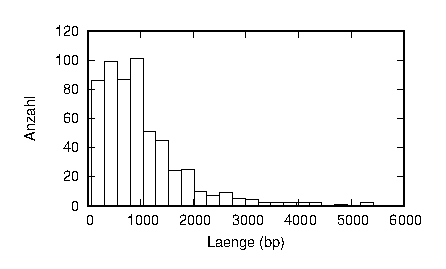
\includegraphics{../gene/hist}
\end{center};
\caption{Die Verteilung von Genlängen im Genom von \emph{M. genitalium}.}\label{fig:hist}
\end{figure}
\nwenddocs{}\nwbegincode{62}\sublabel{NW0-2qU5iO-S}\nwmargintag{{\nwtagstyle{}\subpageref{NW0-2qU5iO-S}}}\moddef{gene.sh~{\nwtagstyle{}\subpageref{NW0-2qU5iO-1}}}\plusendmoddef\nwstartdeflinemarkup\nwprevnextdefs{NW0-2qU5iO-R}{NW0-2qU5iO-T}\nwenddeflinemarkup
awk '\{l=$2-$1+1; print l\}' gene.txt |
    histogram |
    plotLine -x "Länge" -y "Anzahl"
\nwendcode{}\nwbegindocs{63}\nwdocspar
Bisher sind unsere Gene Intervalle auf dem plus oder minus Strang der
DNA. Jetzt wollen wir diese Intervalle sichtbar machen. Wir fangen mit
dem ersten Gen in \ty{gene.txt} an.
\nwenddocs{}\nwbegincode{64}\sublabel{NW0-2qU5iO-T}\nwmargintag{{\nwtagstyle{}\subpageref{NW0-2qU5iO-T}}}\moddef{gene.sh~{\nwtagstyle{}\subpageref{NW0-2qU5iO-1}}}\plusendmoddef\nwstartdeflinemarkup\nwprevnextdefs{NW0-2qU5iO-S}{NW0-2qU5iO-U}\nwenddeflinemarkup
head -n 1 gene.txt
\nwendcode{}\nwbegindocs{65}\nwdocspar
\begin{verbatim}
686     1828    +
\end{verbatim}
Wir verwenden das Programm \ty{drawGenes.awk}, um solche Koordinaten
in Rechtecke zu verwandeln. Der Suffix \ty{awk} im Namen von
\ty{drawGenes.awk} bedeutet, dass es ein Programm in der
Programmiersprache Awk ist. Wir schauen uns den Code an, nur um
festzustellen, dass er lesbarer Text ist.
\nwenddocs{}\nwbegincode{66}\sublabel{NW0-2qU5iO-U}\nwmargintag{{\nwtagstyle{}\subpageref{NW0-2qU5iO-U}}}\moddef{gene.sh~{\nwtagstyle{}\subpageref{NW0-2qU5iO-1}}}\plusendmoddef\nwstartdeflinemarkup\nwprevnextdefs{NW0-2qU5iO-T}{NW0-2qU5iO-V}\nwenddeflinemarkup
cat drawGenes.awk
\nwendcode{}\nwbegindocs{67}\nwdocspar
\begin{verbatim}
{
start = $1
end = $2
strand = $3
...
}
END {
printf "1\t0\n"
}
\end{verbatim}
\nwenddocs{}\nwbegindocs{68}\nwdocspar
Wir verwenden \ty{drawGenes.awk}, um unser erstes Gen in ein Rechteck
zu verwandeln. Dieses besteht aus vier x/y Koordinaten. Die letzte
Position, $(1,0)$, ist unser Ausgangspunkt.
\nwenddocs{}\nwbegincode{69}\sublabel{NW0-2qU5iO-V}\nwmargintag{{\nwtagstyle{}\subpageref{NW0-2qU5iO-V}}}\moddef{gene.sh~{\nwtagstyle{}\subpageref{NW0-2qU5iO-1}}}\plusendmoddef\nwstartdeflinemarkup\nwprevnextdefs{NW0-2qU5iO-U}{NW0-2qU5iO-W}\nwenddeflinemarkup
head -n 1 gene.txt |
    awk -f drawGenes.awk
\nwendcode{}\nwbegindocs{70}\nwdocspar
\begin{verbatim}
686     0
686     1
1828    1
1828    0
1       0
\end{verbatim}
\nwenddocs{}\nwbegindocs{71}\nwdocspar
Diese Koordinate können wir mit \ty{plotLine} plotten, und erhalten
Abbildung~\ref{fig:gene}A.
\begin{figure}
\begin{center}
\begin{tabular}{cc}
\textbf{A} & \textbf{B}\\
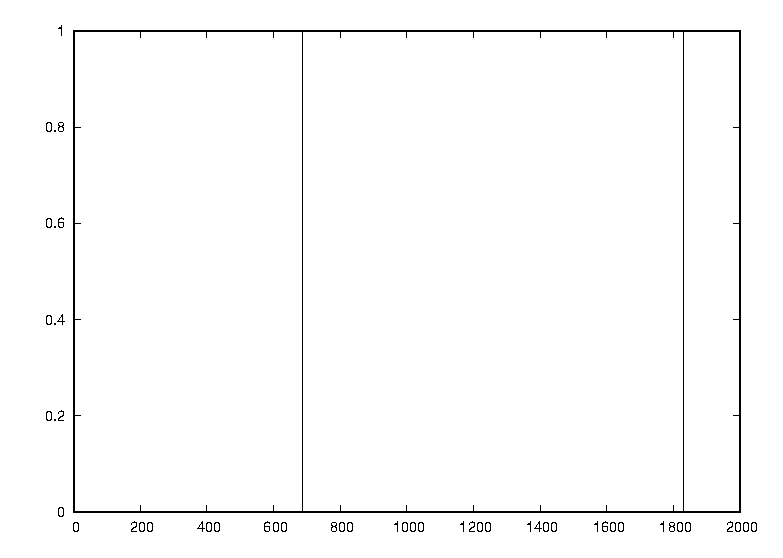
\includegraphics{../gene/gene1} &
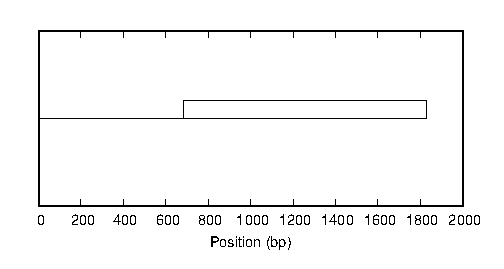
\includegraphics{../gene/gene2}
\end{tabular}
\end{center}
\caption{Erster Versuch, ein Gen zu plotten (\textbf{A}), und zweiter Versuch (\textbf{B}).}\label{fig:gene}
\end{figure}
\nwenddocs{}\nwbegincode{72}\sublabel{NW0-2qU5iO-W}\nwmargintag{{\nwtagstyle{}\subpageref{NW0-2qU5iO-W}}}\moddef{gene.sh~{\nwtagstyle{}\subpageref{NW0-2qU5iO-1}}}\plusendmoddef\nwstartdeflinemarkup\nwprevnextdefs{NW0-2qU5iO-V}{NW0-2qU5iO-X}\nwenddeflinemarkup
head -n 1 gene.txt |
    awk -f drawGenes.awk |
    plotLine
\nwendcode{}\nwbegindocs{73}\nwdocspar
Abbildung~\ref{fig:gene}A ist noch nicht besonders schön. Um sie zu
verbessern, lassen wir die Beschriftung der Y-Achse weg und
verlängern die Y-Achse. Da Gene auf dem negativ-Strang nach unten
gezeichnet werden, machen wir die Y-Achse auch nach oben und unten
symmetrisch. Zuletzt beschriften wir die x-Achse und erhalten
Abbildung~\ref{fig:gene}B.
\nwenddocs{}\nwbegincode{74}\sublabel{NW0-2qU5iO-X}\nwmargintag{{\nwtagstyle{}\subpageref{NW0-2qU5iO-X}}}\moddef{gene.sh~{\nwtagstyle{}\subpageref{NW0-2qU5iO-1}}}\plusendmoddef\nwstartdeflinemarkup\nwprevnextdefs{NW0-2qU5iO-W}{NW0-2qU5iO-Y}\nwenddeflinemarkup
head -n 1 gene.txt |
    awk -f drawGenes.awk |
    plotLine -u y -Y "-5:5" -x "Position"
\nwendcode{}\nwbegindocs{75}\nwdocspar
Jetzt plotten wir alle Gene.
\nwenddocs{}\nwbegincode{76}\sublabel{NW0-2qU5iO-Y}\nwmargintag{{\nwtagstyle{}\subpageref{NW0-2qU5iO-Y}}}\moddef{gene.sh~{\nwtagstyle{}\subpageref{NW0-2qU5iO-1}}}\plusendmoddef\nwstartdeflinemarkup\nwprevnextdefs{NW0-2qU5iO-X}{NW0-2qU5iO-Z}\nwenddeflinemarkup
awk -f drawGenes.awk gene.txt |
    plotLine -u y -Y "-5:5" -x "Position"
\nwendcode{}\nwbegindocs{77}\nwdocspar
Wir merken, die Position ist noch etwas ungeschickt, wir würden sie
gerne von einzelnen Basen in Kilobasen umwandeln. Das können wir auch
mit der Programmiersprache mit der Programmiersprache Awk, die
Zeilenweise vorgeht. In jeder Zeile wird der erste Wert mit \verb+$1+
angesprochen, der zweite Wert mit \verb+$2+, und so weiter. Also
können wir die Positionen von Basen zu Kilobasen umwandeln.
\nwenddocs{}\nwbegincode{78}\sublabel{NW0-2qU5iO-Z}\nwmargintag{{\nwtagstyle{}\subpageref{NW0-2qU5iO-Z}}}\moddef{gene.sh~{\nwtagstyle{}\subpageref{NW0-2qU5iO-1}}}\plusendmoddef\nwstartdeflinemarkup\nwprevnextdefs{NW0-2qU5iO-Y}{NW0-2qU5iO-a}\nwenddeflinemarkup
awk '\{print $1/1000, $2/1000, $3\}' gene.txt |
    head
\nwendcode{}\nwbegindocs{79}\nwdocspar
\begin{verbatim}
0.686 1.828 +
1.828 2.76 +
2.845 4.797 +
4.812 7.322 +
7.294 8.547 +
8.551 9.183 +
9.156 9.92 +
9.923 11.251 +
11.251 12.039 +
12.068 12.724 +
\end{verbatim}

Wir verwandeln die Koordinaten der Gene in Kästchen und plotten sie,
um Abbildung~\ref{fig:genome} zu bekommen.
\begin{figure}
\begin{center}
  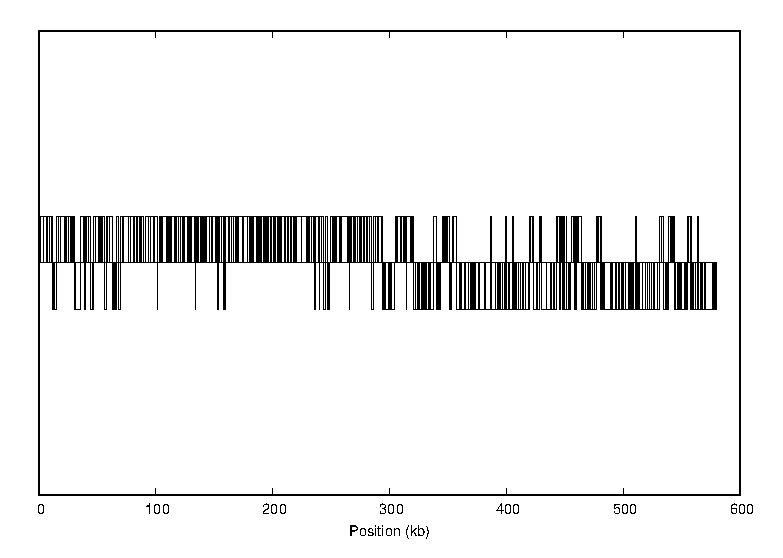
\includegraphics{../gene/genome}
\end{center}
\caption{Die 546 Gene von \emph{M. genitalium}.}\label{fig:genome}
\end{figure}
\nwenddocs{}\nwbegincode{80}\sublabel{NW0-2qU5iO-a}\nwmargintag{{\nwtagstyle{}\subpageref{NW0-2qU5iO-a}}}\moddef{gene.sh~{\nwtagstyle{}\subpageref{NW0-2qU5iO-1}}}\plusendmoddef\nwstartdeflinemarkup\nwprevnextdefs{NW0-2qU5iO-Z}{NW0-2qU5iO-b}\nwenddeflinemarkup
awk '\{print $1/1000, $2/1000, $3\}' gene.txt |
    awk -f drawGenes.awk |
    plotLine -u y -Y "-5:5" -x "Position (kb)"
\nwendcode{}\nwbegindocs{81}\nwdocspar
Wir können die eben erstellte Abbildung auch in einer Datei speichern,
zum Beispiel \ty{genomPlot.eps}. Der Suffix \ty{eps} zeigt an, dass die
Datei im ``encapsulated Postscript'' Format ist.
\nwenddocs{}\nwbegincode{82}\sublabel{NW0-2qU5iO-b}\nwmargintag{{\nwtagstyle{}\subpageref{NW0-2qU5iO-b}}}\moddef{gene.sh~{\nwtagstyle{}\subpageref{NW0-2qU5iO-1}}}\plusendmoddef\nwstartdeflinemarkup\nwprevnextdefs{NW0-2qU5iO-a}{NW0-2qU5iO-c}\nwenddeflinemarkup
awk '\{print $1/1000, $2/1000, $3\}' gene.txt |
    awk -f drawGenes.awk |
    plotLine -u y -Y "-5:5" -x "Position (kb)" -p genomPlot.eps
\nwendcode{}\nwbegindocs{83}\nwdocspar
Wir können unsere neue Postscript Datei mit dem Programm \ty{gv} für
\emph{ghost viewer} anschauen. Das kaufmännische \emph{und}, \verb+&+
am Ende des Befehls öffnet ein unabhängiges Fenster für die Graphik.
\nwenddocs{}\nwbegincode{84}\sublabel{NW0-2qU5iO-c}\nwmargintag{{\nwtagstyle{}\subpageref{NW0-2qU5iO-c}}}\moddef{gene.sh~{\nwtagstyle{}\subpageref{NW0-2qU5iO-1}}}\plusendmoddef\nwstartdeflinemarkup\nwprevnextdefs{NW0-2qU5iO-b}{NW0-2qU5iO-d}\nwenddeflinemarkup
gv genomPlot.eps &
\nwendcode{}\nwbegindocs{85}\nwdocspar
Eine Postscript Datei lässt sich auch gut in eine Textdatei
einbinden. Wir verwenden dazu die Datei \ty{mg.tex}. Der Suffix
\ty{tex} zeit an, dass es sich dabei um eine Datei für das
Setzprogramm \LaTeX{} handelt. Wir schauen uns die Datei an.
\nwenddocs{}\nwbegincode{86}\sublabel{NW0-2qU5iO-d}\nwmargintag{{\nwtagstyle{}\subpageref{NW0-2qU5iO-d}}}\moddef{gene.sh~{\nwtagstyle{}\subpageref{NW0-2qU5iO-1}}}\plusendmoddef\nwstartdeflinemarkup\nwprevnextdefs{NW0-2qU5iO-c}{NW0-2qU5iO-e}\nwenddeflinemarkup
cat mg.tex
\nwendcode{}\nwbegindocs{87}\nwdocspar
\begin{verbatim}
\documentclass{article}
\usepackage{graphics}
\usepackage[german]{babel}
\begin{document}

\title{Meine erste \LaTeX{} Datei}
\author{Beatriz Vieira Mourato}
\maketitle

\begin{center}

\includegraphics{genomPlot}
\end{center}

\end{document}
\end{verbatim}
Wir setzen die Datei als PDF.
\nwenddocs{}\nwbegincode{88}\sublabel{NW0-2qU5iO-e}\nwmargintag{{\nwtagstyle{}\subpageref{NW0-2qU5iO-e}}}\moddef{gene.sh~{\nwtagstyle{}\subpageref{NW0-2qU5iO-1}}}\plusendmoddef\nwstartdeflinemarkup\nwprevnextdefs{NW0-2qU5iO-d}{NW0-2qU5iO-f}\nwenddeflinemarkup
pdflatex mg
\nwendcode{}\nwbegindocs{89}\nwdocspar
Wir schauen das PDF an.
\nwenddocs{}\nwbegincode{90}\sublabel{NW0-2qU5iO-f}\nwmargintag{{\nwtagstyle{}\subpageref{NW0-2qU5iO-f}}}\moddef{gene.sh~{\nwtagstyle{}\subpageref{NW0-2qU5iO-1}}}\plusendmoddef\nwstartdeflinemarkup\nwprevnextdefs{NW0-2qU5iO-e}{\relax}\nwenddeflinemarkup
evince mg.pdf &
\nwendcode{}\nwbegindocs{91}\nwdocspar
Wer mag, kann weiter mit \ty{mg.tex} spielen, den Text verändern, neu
setzen, und so weiter. \LaTeX{} ist von seinem Erfinder Leslie Lamport
schön beschrieben~\cite{lam94:lat}.
\nwenddocs{}

\nwixlogsorted{c}{{gene.sh}{NW0-2qU5iO-1}{\nwixd{NW0-2qU5iO-1}\nwixd{NW0-2qU5iO-2}\nwixd{NW0-2qU5iO-3}\nwixd{NW0-2qU5iO-4}\nwixd{NW0-2qU5iO-5}\nwixd{NW0-2qU5iO-6}\nwixd{NW0-2qU5iO-7}\nwixd{NW0-2qU5iO-8}\nwixd{NW0-2qU5iO-9}\nwixd{NW0-2qU5iO-A}\nwixd{NW0-2qU5iO-B}\nwixd{NW0-2qU5iO-C}\nwixd{NW0-2qU5iO-D}\nwixd{NW0-2qU5iO-E}\nwixd{NW0-2qU5iO-F}\nwixd{NW0-2qU5iO-G}\nwixd{NW0-2qU5iO-H}\nwixd{NW0-2qU5iO-I}\nwixd{NW0-2qU5iO-J}\nwixd{NW0-2qU5iO-K}\nwixd{NW0-2qU5iO-L}\nwixd{NW0-2qU5iO-M}\nwixd{NW0-2qU5iO-N}\nwixd{NW0-2qU5iO-O}\nwixd{NW0-2qU5iO-P}\nwixd{NW0-2qU5iO-Q}\nwixd{NW0-2qU5iO-R}\nwixd{NW0-2qU5iO-S}\nwixd{NW0-2qU5iO-T}\nwixd{NW0-2qU5iO-U}\nwixd{NW0-2qU5iO-V}\nwixd{NW0-2qU5iO-W}\nwixd{NW0-2qU5iO-X}\nwixd{NW0-2qU5iO-Y}\nwixd{NW0-2qU5iO-Z}\nwixd{NW0-2qU5iO-a}\nwixd{NW0-2qU5iO-b}\nwixd{NW0-2qU5iO-c}\nwixd{NW0-2qU5iO-d}\nwixd{NW0-2qU5iO-e}\nwixd{NW0-2qU5iO-f}}}%



\bibliography{ref}
\end{document}

